\documentclass[UTF8]{ctexart}
\usepackage{float}
\usepackage{graphicx}
\usepackage{listings}
\usepackage{xcolor}
\CTEXsetup[format={\Large\bfseries}]{section}
\pagestyle{plain}
\title{\normalsize
\LARGE    
DDNL

Assignment 4
}
\author{\
    程琪聪\\
    2153834
}
\date{\today}

\lstset{
    language=SQL,
    basicstyle=\ttfamily,
    breaklines=true
}

\begin{document}
\maketitle
\section{解释一下 RNN ,LSTM,GRU模型.}
\subsection{循环神经网络(RNN)}
RNN 是一种经典的神经网络架构,其特点在于具有循环连接,允许信息在网络内部进行持续传递。这使得 RNN 能够处理序列数据,并且对于具有时间相关性的数据,如时间序列或文本等非常有效。

然而,传统的 RNN 存在梯度消失和梯度爆炸等问题,这些问题限制了 RNN 在处理长序列时的效果。为了解决这些问题,出现了一些改进的 RNN 变体,其中最著名的是 LSTM 和 GRU。
\subsection{长短期记忆网络(LSTM)}
长短期记忆网络是一种特殊类型的 RNN,旨在克服传统 RNN 中的长期依赖问题。LSTM 引入了三个门控结构:遗忘门、输入门和输出门,以及一个内部状态单元。这些门控结构允许 LSTM 有选择地忘记、记忆或输出信息,从而有效地处理长期依赖关系。LSTM 通过学习何时更新其内部状态以及何时忘记信息,使其能够更好地捕捉序列中的长期模式。
\subsection{门控循环单元(GRU)}
门控循环单元是另一种改进的 RNN 变体,旨在简化 LSTM 并减少其参数数量。与 LSTM 类似,GRU 也具有更新门和重置门,但合并了状态和输出,并且没有单独的内部状态单元。GRU 相对于 LSTM 更容易训练,并且具有更少的参数,因此在一些场景下可能更受欢迎。
\subsection{比较}
\begin{itemize}
    \item LSTM 比传统的 RNN 效果更好,尤其是在处理长序列时,因为它能够更好地捕捉长期依赖关系。
    \item GRU 是对 LSTM 的一种简化,具有更少的参数和门控结构,因此在某些情况下训练速度更快,同时效果也可以与 LSTM 相媲美。
\end{itemize}

\section{叙述一下 这个诗歌生成的过程。}
\subsection{数据预处理}
程序首先从文本文件中读取诗歌数据,并进行预处理,包括去除特殊符号、标点符号,以及长度过长或过短的诗歌。将每首诗歌转换为一个向量,其中每个字被映射为一个整数索引。同时建立一个字典,将每个字映射到其对应的整数索引。
\subsection{模型构建}
该程序中使用了一个简单的RNN模型,包括一个嵌入层(embedding layer)和一个RNN层。嵌入层将每个字的整数索引转换为密集的向量表示。RNN层接收嵌入向量序列作为输入,并输出下一个字的预测结果。
\subsection{训练模型}
使用生成的批量数据进行模型的训练。每个批次包含多个诗歌向量,其中每个诗歌向量由一串字的整数索引组成。模型的训练目标是最小化损失函数,损失函数衡量模型的预测结果与实际下一个字的差异。
\subsection{生成诗歌}
训练完成后,可以使用模型生成新的诗歌。用户指定一个开始的字作为输入,并通过模型预测接下来的字,逐步生成一首完整的诗歌。
\section{训练及生成结果}
\begin{figure}[H]
    \centering
    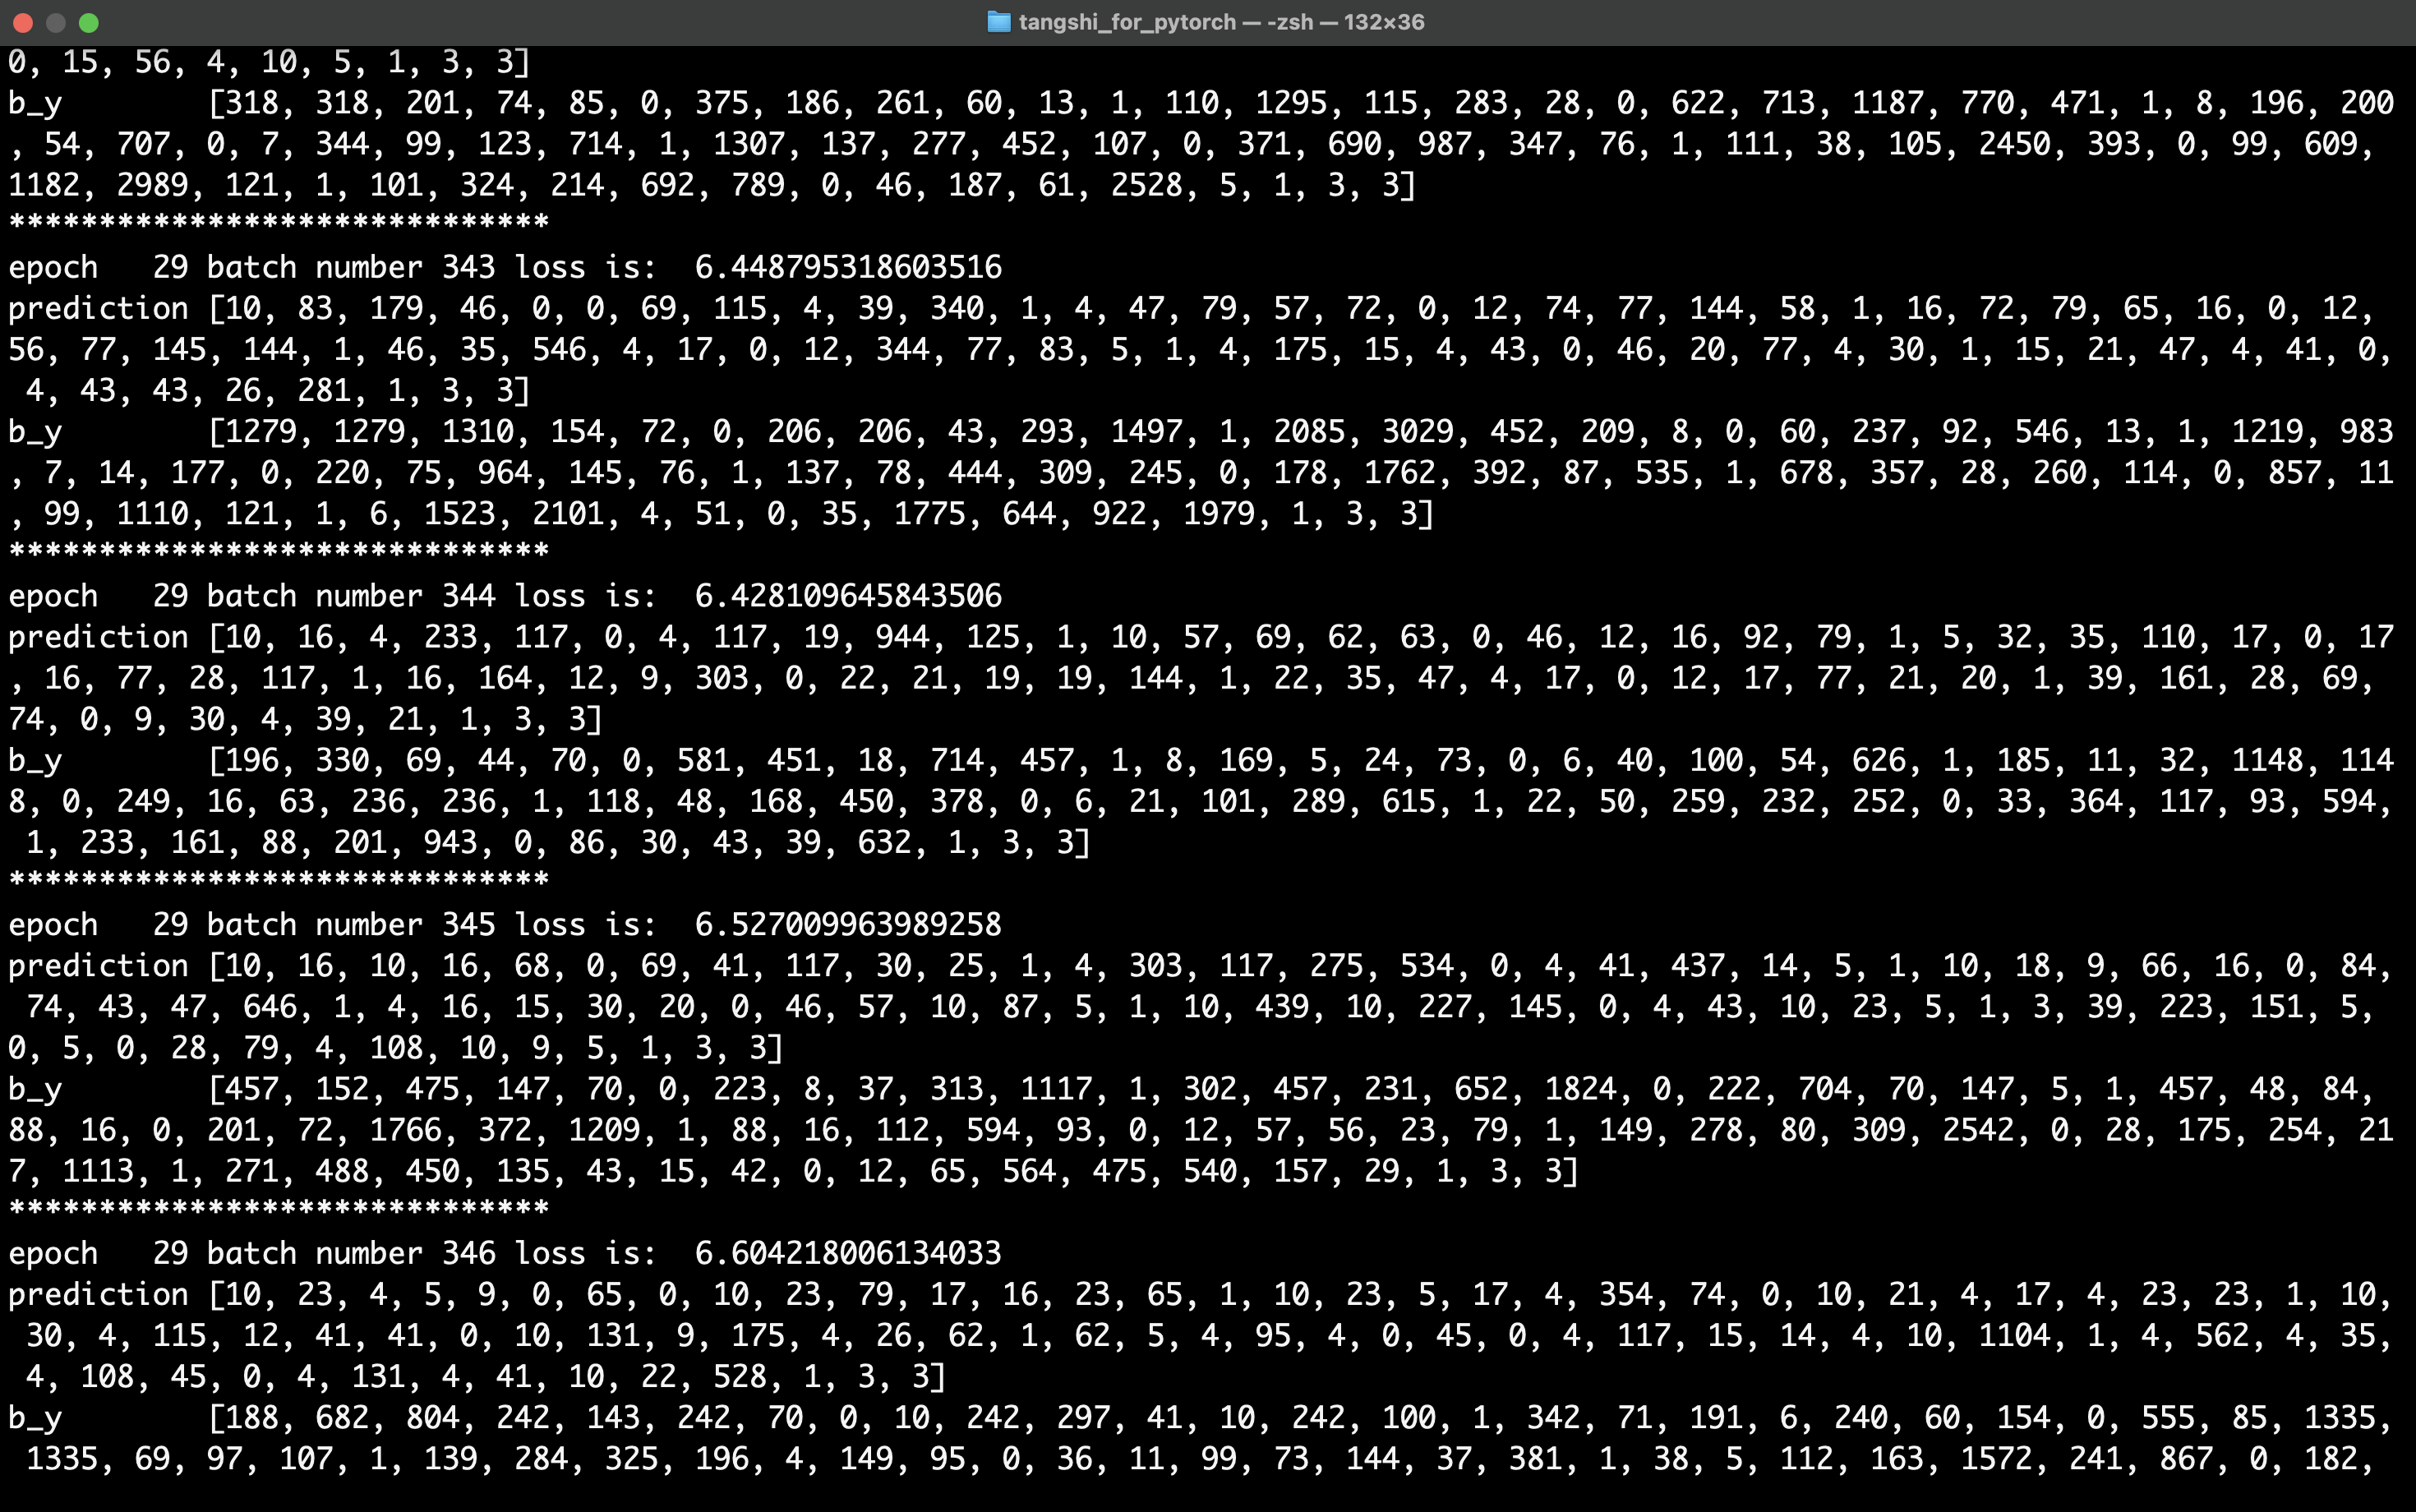
\includegraphics[width=0.7\textwidth]{./assets/1.png}
    \caption{训练过程}
    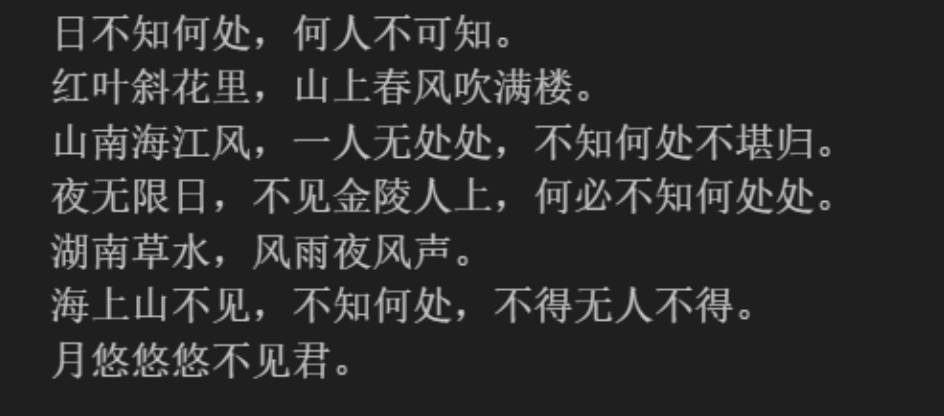
\includegraphics[width=0.7\textwidth]{./assets/2.png}
    \caption{生成结果}
\end{figure}
\end{document}